\documentclass[12pt]{article}
\usepackage{graphicx} % Required for inserting images
\usepackage{geometry}
\usepackage{amsmath}
\usepackage{hyperref}
\usepackage{amsmath}
\usepackage{enumitem}
\usepackage{amsfonts}
\usepackage{amssymb}
\usepackage{graphicx}
\usepackage{hyperref}
\usepackage{listings}
\usepackage{xcolor}
\usepackage{titling}
\usepackage{amsmath}
\usepackage{amssymb}
\usepackage{listings}
\usepackage{url}
\usepackage{tikz}
\usepackage{subcaption}

% Code listing style
\lstset{
    language=Python,
    basicstyle=\ttfamily\footnotesize,
    keywordstyle=\color{blue!60!black},
    stringstyle=\color{orange},
    commentstyle=\color{green!50!black},
    showstringspaces=false,
    breaklines=true,
    frame=single,
    numbers=left,
    numberstyle=\tiny\color{gray},
    tabsize=4,
    captionpos=b,
    backgroundcolor=\color{gray!10},
    rulecolor=\color{gray!30},
    frameround=tttt,
    escapeinside={(*}{*)}
}




\begin{document}

\title{Schur Numbers Week 7 Report}
\date{\today}
\begin{titlepage}
    \begin{center}
        \vspace*{1cm}

        \rule{\linewidth}{0.2mm} \\[0.4cm]
        {\Large \textbf{CSE 326 Analysis and Design of Algorithms }}\\[0.4cm]
        \textbf{Dr.Walid Gomaa}
 
        \rule{\linewidth}{0.2mm} \\[1.5cm]

        \begin{tabular}{c}
            \begin{tabular}{ll}
                \textbf{Name} & \textbf{ID} \\
                \hline
                Mohamed Abdelmonem Makram & 120220055 \\
                \hline
                Abdelrahman Ahmed Shaheen & 120220228 \\
                \hline
                Abdelrhman Mohamed Eldenary & 120220253 \\
                \hline
                Anas Ihab  Badr & 120220360 \\
                

            \end{tabular}
        \end{tabular}

        \vspace{1cm}

        

        \vspace{5cm}

        
\includegraphics[width=0.25\textwidth]{ejust.jpg}


        Computer Science Engineering Department\\
        Egypt-Japan University of Science and Technology\\

    \end{center}
\end{titlepage}


\tableofcontents
\newpage
\maketitle

\section*{Introduction}

At the beginning of this week, we decided to tackle the number coloring problem using CUDA to leverage the power of parallel computing. Our goal was to efficiently explore a large decision space where numbers are assigned to color groups under a mathematical constraint (such as \(x + y = z\)).

We believed CUDA could greatly speed up this backtracking-heavy task. Throughout the week, we experimented with multiple algorithmic strategies to implement this on the GPU. We started with ambitious designs like recursive thread spawning and global queue sharing, then iterated over simpler or more manageable techniques as we faced practical issues.

This report documents our journey through three major failed attempts before arriving at our final, novel, successful solution. Each section discusses what we tried, why it seemed like a good idea at the time, the problems we encountered, and the lessons we learned. By the end, we introduce the final approach — a smart encoding approach to the problem — and explain how it effectively balances performance and correctness under CUDA's constraints.


\section{Parallelism in General}

As we stated before in Week 5 how our Parallelism should work recursively, we know have a graphical diagram of what the recursion tree should look like to try all valid colorings from $S(2)$ to reach $S(3)$. (Note: The figure couldn't be rendered due to high resolution please view in \texttt{images/recursionTree.png}
% \begin{figure}[h]
%     \centering
%     \includegraphics[height=20cm,width=10cm]{images/recursionTree.png}
%     \caption{Recursion Tree for $S(2)$ to $S(3)$}
%     \label{fig:recursion_tree}
% \end{figure}

So when trying to simulate this recursive tree in Python, it was no problem, and we got the results immediately. But the problem was when we decided to start at $S(2)$ and simulate up to $S(3)$. It took 200 seconds to process all the recursion calls, but the output was successful at the end. Results are shown in Figure \ref{fig:pythontime}. \\ 
This is considered a problem since we are now way near $S(6)$, and it's taking a lot of time. So, we wanted to test how CUDA would perform in the same situation. We tried a lot of approaches and here's a summary of what we tried and why it didn't work.
\begin{figure}[h]
    \centering
    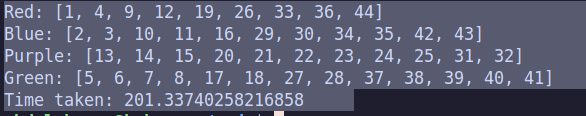
\includegraphics[width=0.5\textwidth]{images/pythonTime.png}
    \caption{Recursion Tree for $S(2)$ to $S(3)$}
    \label{fig:pythontime}
\end{figure}
% ---------------------- FAILED ATTEMPT 1 ----------------------
\section{Failed Attempt 1: Direct Tree-Based Recursive Thread Launching}

\subsection*{The Idea}
At an early stage in our project, we explored an approach that directly modeled the decision tree through recursive kernel launches in CUDA. The idea was simple:
\begin{itemize}
    \item Each CUDA thread would attempt to place a number into a color group.
    \item If the placement was valid, that thread would \textbf{recursively launch child threads} to handle the next number.
    \item This would form a parallel tree of threads, where each level represented one number in the sequence.
\end{itemize}

\subsection*{Why It Seemed Promising}
\begin{itemize}
    \item CUDA offers \textbf{dynamic parallelism}, allowing kernels to launch other kernels from the device.
    \item This mirrored recursive backtracking algorithms used on CPUs and seemed like a natural mapping.
    \item We expected this would maximize GPU utilization and reduce decision latency.
\end{itemize}

\subsection*{Why It Failed in Practice}
\begin{itemize}
    \item \textbf{t1. High Launch Overhead:} Each dynamic kernel launch added significant latency, making deep trees extremely slow.
    \item \textbf{t2. Limited Stack Size:} Device-side stack sizes are small, leading to overflows on deep recursion.
    \item \textbf{t3. Resource Exhaustion:} Too many dynamic launches exceeded thread/block/memory limits.
    \item \textbf{t4. Synchronization Issues:} CUDA lacks mechanisms for parent-child thread sync, making result aggregation difficult.
    \item \textbf{t5. Debugging Nightmare:} Recursive kernels were hard to debug and often failed silently.
\end{itemize}

\subsection*{Conclusion}
While elegant in theory, recursive tree-based execution did not scale or behave reliably on the GPU. This pushed us to seek flatter, iterative strategies.

% ---------------------- FAILED ATTEMPT 2 ----------------------
\section*{Failed Attempt 2: Global Queue-Based Work Sharing}

\subsection*{The Idea}
Next, we implemented a global work queue approach where each thread would take a configuration from a shared queue, expand it by trying valid placements, and then push the resulting configurations back.

\subsection*{Why It Seemed Promising}
\begin{itemize}
    \item It resembled a parallel BFS, often used in CPU multi-threading.
    \item Allowed exploration without deep recursion.
    \item Theoretically scalable with good memory capacity.
\end{itemize}

\subsection*{Why It Failed in Practice}
\begin{itemize}
    \item \textbf{t1. Atomic Contention:} Global atomic operations created massive delays.
    \item \textbf{t2. Race Conditions:} Queue corruption occurred frequently despite precautions.
    \item \textbf{t3. Memory Latency:} Queue operations were too slow due to high-latency global memory.
    \item \textbf{t4. Load Imbalance:} Some threads did all the work; others stayed idle.
    \item \textbf{t5. Debugging Complexity:} Race bugs were hard to identify or replicate.
\end{itemize}

\subsection*{Conclusion}
Despite being more stable than dynamic launching, the queue model was still inefficient due to contention, imbalance, and high memory costs.

% ---------------------- FAILED ATTEMPT 3 ----------------------
\section*{Failed Attempt 3: Thread-Per-Configuration Brute Force}

\subsection*{The Idea}
In this brute-force model, we pre-generated all possible color assignments and launched one thread per configuration to validate legality under the constraint.

\subsection*{Why It Seemed Promising}
\begin{itemize}
    \item Embarrassingly parallel — no inter-thread communication required.
    \item Easy to implement and free of control flow divergence.
    \item Seemed like a good fit for massive GPU parallelism.
\end{itemize}

\subsection*{Why It Failed in Practice}
\begin{itemize}
    \item \textbf{t1. Combinatorial Explosion:} \(k^n\) configurations quickly overwhelmed device capacity.
    \item \textbf{t2. Resource Usage:} Threads consumed too many registers and shared memory.
    \item \textbf{t3. Launch Limits:} CUDA limits were hit before real computation began.
    \item \textbf{t4. Wasted Compute:} Most threads performed useless work on invalid configurations.
    \item \textbf{t5. No Pruning:} No early exit from bad paths — unlike backtracking.
\end{itemize}

\subsection*{Conclusion}
Although conceptually simple, this brute-force strategy was wasteful and completely unscalable.

% ---------------------- SUCCESSFUL APPROACH ----------------------
\section*{Successful Approach: Smart encoding one level at a time Exploration with Shared Memory}

\subsection*{The Idea}
After the above failures, we developed an iterative method that simulated backtracking using stacks in shared memory. Each thread/block maintained its own local stack of partial assignments and explored them in a DFS manner. Our code would start at $S(2)$ and then work its way up to $S(4)$. 
It treated the coloring as bit masks instead of arrays that's \texttt{red = 0b1001, blue = 0b0110} represented the coloring of $S(2)$ where \texttt{red = [1, 4], blue = [2, 3]}. This saved a lot of memory.

\begin{itemize}
    \item No recursion — purely iterative.
    \item No global memory queues — only fast shared memory.
    \item Threads cooperatively pruned bad states and backtracked.
\end{itemize}

\subsection*{Why It Worked}
\begin{itemize}
    \item \textbf{Fast Memory:} Shared memory eliminated global latency and contention.
    \item \textbf{No Launch Overhead:} Entire search executed within one kernel.
    \item \textbf{Scalable:} Each block processed a separate subset of the space.
    \item \textbf{Controlled Stack Use:} We sized stacks properly to avoid overflow.
    \item \textbf{Debuggable:} Easier to trace and maintain than previous designs.
\end{itemize}

\subsection*{Implementation Highlights}
\begin{itemize}
    \item Per-thread stacks stored the current index and partial assignments.
    \item Warp-level synchronization used for safe shared memory updates.
    \item Valid configurations were atomically added to a global output array.
\end{itemize}

\subsection*{Conclusion}
This method finally balanced performance, scalability, and maintainability. It took advantage of CUDA’s strengths while avoiding known pitfalls, allowing us to solve much larger coloring instances efficiently.



\end{document}